\documentclass[11pt,a4paper]{article}

% [†ONT-MS] METRIC-SINGULARITY FORCING — this paper is the HOME (ONTOLOGY_FOUNDATION_INDEX.md §1c).
%   ARC POSITION (THE_EVOLUTION_MAP.md): this is where the corpus's ontological forcing BEGINS, and it
%   STANDS ON STANDARD GENERAL RELATIVITY ALONE — no substrate, no foliation, no augmentation, no
%   reassignment. Its corpus citations are NEVER dependencies: they are forward pointers, plus the
%   ADJACENT-AND-NEGATIVE citation of P4 (§318 names P4 precisely to disclaim reliance on it — "the
%   present paper reaches the distinction from standard general relativity alone"), which P4 returns in
%   kind (P4 §109/§196: this result "stands on causal structure alone and needs none of the cosmological
%   evidence"). THE TWO KEYSTONES ARE DELIBERATELY NON-LOAD-BEARING ON EACH OTHER: P1 supplies the
%   STRUCTURAL half of the augmentation's necessity, P4 the EMPIRICAL half, and because neither leans on
%   the other their convergence is EVIDENCE rather than construction — a dependency between them would
%   make the necessity circular. This is structurally essential, not modesty: the first result must not
%   LEAN ON what the arc later builds. But the forbidden thing is LEANING FOR SUPPORT, not reference: P1's
%   logic owes the arc nothing, which is exactly what lets the arc draw on P1 WITHOUT circularity, and
%   adjacent-and-negative forward references (disclaiming reliance while naming what P1 supplies) are fine
%   — P1<->P4 already does this, and P1<->P6 now does it for the imperative. Its own floor is an EPISTEMOLOGY
%   OF CAUSAL KNOWLEDGE (only the fixed causal past yields certain information — the M31 V1 example), and
%   that floor is itself a BESPOKE INSTANCE of P6's imperative, reached on causal structure alone: so P1
%   does not "need no epistemic ground and is given none" — it SUPPLIES one, bespoke, that P6 draws on
%   reciprocally. The rule: do not reach forward FOR SUPPORT; P1 owes the arc nothing for its LOGIC.
%   Masthead / established here (the taproot; presupposes only standard Lorentzian GR — this is where
%   CR's ontological forcing BEGINS): the metric singularity is a forced third category (null +
%   spatially-coincident along the connection => zero temporal separation, causal order intact; NOT a
%   coordinate singularity, NOT a manifold singularity, NOT an ordinary null hypersurface); the event
%   horizon IS one (any Killing horizon); it occurs only as the null future boundary at infinite
%   exterior time, every exterior "now" asymptotically tangent to a single generator; densities never
%   form. Roots downstream: the cosmogenesis branch point, which IS r=0 (r2154; the earlier "not r=0" here
%   was the pre-r2154 belief that it sat at the Nariai seam a full lap away). It is finite-curvature in the
%   sense P16 states: the throat IS alpha, so the r-chart divergence is the AREAL COORDINATE degenerating,
%   not a curvature scale of the substrate. Also downstream: the reassignment of the
%   limiting generator as cosmic time (P7), the throat that IS alpha, the substrate's defining constant (P3/P8) — see §1c.

\usepackage[margin=1in]{geometry}
\usepackage{amsmath, amssymb, amsthm}
\usepackage{mathtools}
\usepackage{mathrsfs}
\usepackage{graphicx}
\usepackage[dvipsnames]{xcolor}
\usepackage{hyperref}
\usepackage{caption}
\usepackage{receipts}
\usepackage{ledgers}  % in-place receipt citations -> Appendix R

\hypersetup{
  colorlinks=true,
  linkcolor=blue!50!black,
  citecolor=blue!50!black,
  urlcolor=blue!50!black
}

\theoremstyle{plain}
\newtheorem{theorem}{Theorem}
\newtheorem{corollary}{Corollary}
\newtheorem{lemma}{Lemma}
\newtheorem{proposition}{Proposition}
\theoremstyle{remark}
\newtheorem{remark}{Remark}

\captionsetup{font=small, labelfont=bf}

\title{The event horizon is a metric singularity:\\
\large a missing definition in general relativity, and the black-hole problems it dissolves}
\author{Daryl Janzen\\
\small Department of Physics and Engineering Physics\\
\small University of Saskatchewan}
\date{}
\newcommand{\dd}{\mathrm{d}}   % r2376+c54.9: used but undefined -- the paper did not compile
\begin{document}
\maketitle

\begin{abstract}
We identify a geometric structure we argue standard general relativity has lacked among its
standard definitions: the \emph{metric singularity}---a null hypersurface along whose
generators the spatial extent has, in addition, contracted to zero, so that events on a
generator are topologically distinct and causally ordered yet carry no metric separation. Using only
standard Lorentzian structure, we prove a Metric Singularity Theorem: two events that
are both null-separated and spatially coincident have vanishing temporal separation as
well; two of the three separations vanishing forces the third. We distinguish this
sharply from the generic case: an ordinary null hypersurface, such as an observer's
past light cone, carries frame-dependent but nonzero temporal separations and is
\emph{not} a metric singularity. Specializing to the Schwarzschild geometry, we show
that the future event horizon $\mathcal{H}^+$ satisfies the theorem's hypotheses---horizon-crossing events on a common generator occur at the same areal radius $r_h$, hence at zero invariant spatial separation---and is therefore a metric singularity. The same forcing extends the conclusion to any Killing horizon, the Kerr family included. Independently of this metric identification, the horizon's defining causal property---that it is the null future boundary of the exterior, $\mathcal{H}^+=\partial J^-(\mathscr{I}^+)$---forces any temporal slicing adapted to an exterior observer to become asymptotically tangent to a single horizon generator and to meet $\mathcal{H}^+$ only in the limit of infinite exterior time:
within the causal domain of the external universe, the event horizon occurs solely as a
null future boundary approached asymptotically by every admissible ``now'' slicing. This
clarifies the behavior of horizon neighborhoods in Eddington--Finkelstein diagrams,
constrains the interpretation of horizon-proximal processes in gravitational collapse,
and implies that the densities associated with the central singularity never form at any
finite exterior time. Because the globally completed horizon on which the standard black-hole problems rest is, for this reason and in a universe of ongoing mergers and accretion, never physically realised, three of those problems dissolve on causal grounds alone and are drawn out here: no closed trapped surface is realised, so Penrose's singularity theorem, though mathematically correct, has physical preconditions the astrophysical domain never meets, and cosmic censorship becomes unnecessary; the horizon-induced Bogoliubov\ldg{functional_analysis} mode-splitting that yields Hawking radiation has no realised background to be computed on, leaving \emph{horizon-induced} radiation absent while local, non-horizon particle production is untouched; and the information-loss paradox does not arise, the realised spacetime remaining globally connected, with a global Cauchy surface and unobstructed unitary evolution. Each of these follows from the same standard causal structure and no modification of general relativity.
\end{abstract}

\section{Null separation, non-invariance, and metric singularities}\label{sec:1}

Black-hole physics has for half a century built its central results---the singularity theorems, Hawking radiation, the information paradox---on a reading of the event horizon as a removable coordinate artefact: a surface a suitable chart passes through smoothly, behind which a completed interior and a curvature singularity are taken to lie. This paper supplies a definition that reading has lacked, and corrects it. We identify a geometric structure standard general relativity does not name among its own---the \emph{metric singularity}, a null hypersurface along whose generators the spatial extent has, in addition, contracted to zero---and prove that the event horizon is one. It is not a coordinate artefact but a locus at which the metric's spatial measure collapses; and, being the null future boundary of the exterior, it \emph{occurs} without ever \emph{existing} on any finite exterior-time slice, so that the densities of the central singularity never form at finite exterior time. The completed, physically realised horizon on which the standard problems rest is therefore never instantiated in a universe of ongoing collapse and accretion, and three of those problems---the singularity theorems, Hawking radiation, and the information paradox---dissolve on causal grounds alone, with no modification of general relativity. The whole argument uses nothing but standard Lorentzian and causal structure; we reach its central definition first by following an elementary limit, beginning with what an observer in relativity can and cannot know about a distant object.

According to general relativity, there is a fundamental distinction between the events contained within an observer's fixed causal past---defined by the interior of their past light cone---and events that are merely ``past'' according to some arbitrary coordinate slicing but are spacelike separated from the observer. Only the former constitute physically certain information; the latter do not admit invariant temporal status relative to the observer.

For example, consider M31~V1, a Cepheid variable in the Andromeda galaxy~\cite{Hubble1929M31}. In our fixed causal past, M31~V1 is observed as a bright, evolved supergiant. The fact that we see it as such today implies that the star must have previously formed and undergone stellar evolution to reach this phase before the light we now observe was emitted.

However, Andromeda lies roughly $2.5$ million light-years away. What we observe ``now'' is M31~V1 as it was $2.5$ million years ago. M31~V1 may well have already undergone a core-collapse supernova sometime within the past $2.5$~million years; yet we do not possess causal knowledge of that event. The reason is formal: the putative M31~V1 supernova is spacelike separated from here-now. Therefore, no positive statement about whether that explosion has already occurred (in any absolute sense) is meaningful without adopting a specific relativistic coordinate convention.

Thus, an observer's fixed causal knowledge in relativity is constrained entirely by the past light cone. The physical state we ascribe to distant astronomical objects is necessarily based on the most recent event in our causal past, which depends on their lookback distance. No astronomer refers to M31~V1 as ``a supernova remnant,'' although that may well be its status on a natural cosmological time slicing; rather, we may only say with certainty what it was when it emitted the photons that currently reach Earth. The same constraint, we will see, applies to a verb form that has propagated through fifty years of horizon literature: speaking of a black hole as a ``collapsed object'' presupposes a past-tense status that the horizon's causal structure does not licence.\footnote{This epistemology of causal knowledge---only the fixed causal past yields certain information, so an appearance is not the present state of the world it images---is a bespoke instance of an inference a companion foundation later sets out in general (do not take the appearance at face value; infer the world it arises from)~\cite{JanzenShadowExistence}, and it is not the only such instance here. The same discipline, reached on causal structure alone, recurs through the paper: that the metric's verdict of coincidence is a fact about the ruler and not the identity of the events it separates only in null order (\S\ref{sec:2}) is a projection read as a projection---here a \emph{real} projection, not an illusory one; that ``collapsed'' presupposes what the geometry does not licence, so \emph{the grammar must follow the geometry} (\S\ref{sec:4}), is ontology read from the evidence rather than off a reified coordinate---the reification error caught in a verb tense; and that the standard black-hole problems dissolve once the premise they rest on is seen never to be instantiated (\S\ref{sec:problems}) is dissolution by identity, not by patchwork. Each is reached here without the general treatment, and that independence is exactly what lets the general account draw on these instances without circularity---the same non-leaning relation this paper holds to the empirical keystone it converges with~\cite{JanzenModernParallax}.}

This causal structure has a consequence for the temporal relation between null-separated events that is easy to half-state and thereby get wrong, and the distinction we draw now is the one on which the rest of the paper turns. Consider two events $p$ and $q$ on a single future-directed null geodesic---a photon's emission and its later reception, say. They are distinct points of the manifold; they are causally ordered, $p$ before $q$; and their \emph{spacetime} separation is zero, because the geodesic joining them is null. The question is what this says about their \emph{temporal} separation, and the answer has two parts that must not be merged.

First, the temporal separation $\Delta\tau=\tau(q)-\tau(p)$ assigned by a smooth temporal function $\tau$ is not a geometric invariant. Different admissible temporal functions assign different values; a boost changes it; it is frame-dependent. This is true of \emph{every} null-separated pair, and it is all that holds in general.

Second---and this is the part that is easy to overstate---non-invariance is \emph{not} degeneracy. That $\Delta\tau$ is frame-dependent does not mean it can be driven to zero. The photon emitted from the far side of the Andromeda galaxy and received here now is null-separated from its emission, causally ordered, and topologically distinct; its temporal separation is frame-dependent, yet in no admissible frame is it anything but enormous. The reason is that $p$ and $q$ are separated by a large \emph{spatial} distance---some two and a half million light-years---and an ordinary null pair carries exactly this nonzero spatial separation. A generic null geodesic, and a generic null hypersurface such as one's past light cone, is null in its spacetime interval while remaining spread over nonzero spatial extent. Its events are not metrically coincident.

What makes the temporal separation collapse is an \emph{additional} condition: that the spatial separation vanish as well. This is a special circumstance, not the generic one, and it is the circumstance the event horizon will turn out to realize. To see the condition built up as a limit before stating it as a theorem, it is worth following a thought experiment.

The Andromeda galaxy spans roughly $100\,\mathrm{kly}$ in the radial direction relative to Earth. Consequently, the image we observe is not Andromeda ``as it is now,'' nor even ``as it was exactly $2.5$ million years ago.'' Instead, we receive light whose emission times vary by $\sim10^5$~years across the radial extent: photons originating on the far side were emitted roughly $\sim10^5$~years earlier than those from the near side. As light propagates along the null geodesic connecting those regions to us, photons emitted from progressively nearer regions join the same bundle of null generators; the image we observe is the accumulated result of this continual inflow of successively later emission events.

Now imagine a hypothetical scenario in which Andromeda contracts along the radial direction, bringing its near and far sides increasingly close together, asymptotically approaching coincidence in the infinite future. In that limit, photons from the near and far regions would ultimately arrive from exactly the same spatial location in our past light cone. Their emission events remain distinct and causally ordered---the far-side emission event precedes the near-side emission event along a null geodesic connecting the two---yet their spatial separation in our frame vanishes. As the spatial separation contracts to zero while the null relation is maintained, the two emission events become coincident in both a practical and a metrical sense, even though they remain topologically distinct and causally ordered. The set of emission events, and their order, is preserved entire; only the geometry laid over the set collapses.

Crucially, the construction does not require that the worldlines hosting these emission events remain nonsingular in the future. Even if either or both regions of Andromeda encounter a curvature singularity at some later time, as long as the segment of spacetime in the causal past of the relevant null geodesic is smooth, the result holds without modification.

A second construction, with no light and no geometry in it at all, reaches the same object and is worth setting beside the first. Picture a row of runners aimed at a wall---idealised as a single point of space at which all the runners arrive---spaced out behind one another along the common approach line: one at $10$ metres, one at $100$ metres, one at a kilometre, and so on, as far back as you like. Let each runner's speed be conditioned on both how far from the wall they are and what time it is, tuned so that every runner reaches the wall at the same instant. There is nothing exotic in this; it is an ordinary rule assigning a speed to each runner at each position and time, and one can write it down explicitly. To see what it forces, take the extreme case: the runner a kilometre out and the runner at $10$ metres cross the finish together, so over the final stretch the distant runner---who began far faster---must have its speed driven smoothly toward zero, slowing without limit as the wall approaches, so as not to arrive early. Push the starting line farther back, to a light-year, and the effect only sharpens: the farthest runner spends almost the entire race shedding speed, arriving neither sooner nor later than the one that started a step away. The single extreme case settles the whole row at a glance. Every arrival happens at the wall, at one instant.

And now read off the three properties without any computation. The arrivals are topologically distinct: different runners, distinct in identity and origin---each having travelled its own path from its own starting distance. They are causally ordered: traced back along the approach, the near runner's arrival precedes the next, which precedes the next, in a definite sequence---exactly the order an Eddington--Finkelstein diagram would display. And they are metrically coincident: all arrivals occur at the wall, at one instant, with no spatial and no temporal separation between them. The causal order is real; the metrical separation is not. Position alone would not do this---runners at fixed speeds and different distances arrive at different times---it is the conditioning of speed on \emph{time} as well as position that forces the coincident arrival. The Andromeda limit builds the structure optically, by contracting the spatial depth of an image to zero; the wall builds it kinematically, by driving approach speeds to zero separation at the instant of arrival. They are the same object, reached two ways.

Both constructions exhibit one structure, and it is worth saying plainly what it is, because it invites the very misreading the rest of the paper turns on dispelling. In each, a set of genuinely distinct events---distinct emission events across the galaxy's depth; distinct runners of distinct origin---is assigned, by the measure laid over it, a single place at a single instant. The distinctness is a fact about the events; the coincidence is a fact about the ruler. To read ``one place, one instant'' as ``therefore one event'' is to mistake the place the metric assigns for the identity of the points it assigns it to---and a place is not a point. A metric can collapse every separation it measures and still not merge events it did not individuate, nor revoke an order it does not carry, for it did not lay the set down. This is not a defect of the constructions to be cleared away; it is the object the paper names---distinct, ordered points at one place. The Schwarzschild horizon of Section~\ref{sec:3} is shown to be the same object once more, reached a third way, by the geometry itself: what the optical and kinematic limits approach, the horizon realises exactly.

We now isolate the condition these two constructions share as a theorem. It is the central definition of this paper, and---once both its hypotheses are in view---it is trivially provable. The triviality is the point: it identifies, with no machinery, exactly the extra condition that turns an ordinary null relation into a metrically singular one.

\begin{theorem}[Metric Singularity]\label{thm:metric-singularity}
Let $(M,g)$ be a smooth Lorentzian manifold and let $p,q\in M$ be two events that are
\begin{enumerate}
\item[(a)] \emph{null-separated}: their spacetime interval vanishes, $\Delta s^2=0$; and
\item[(b)] \emph{spatially coincident}: their invariant spatial separation vanishes, $\Delta x=0$, in the sense that $p$ and $q$---and every point of the null geodesic joining them---share the same value of an invariantly-defined spatial coordinate, so that no frame adapted to the corresponding foliation assigns them a spatial separation.
\end{enumerate}
Then their temporal separation vanishes also, $\Delta\tau=0$. The events $p$ and $q$ are \emph{metrically coincident}---the metric assigns no nonzero separation between them---spatial, temporal, or spacetime---while remaining, in general, topologically distinct and causally ordered.
\end{theorem}

\begin{remark}
Hypothesis (b) is, as stated, a condition along the whole connection: the connecting null geodesic remains at the common value of the invariant spatial coordinate, not merely its endpoints. This along-the-connection form is what the passage from the metric relation among the invariant separations to a vanishing finite temporal separation requires when $p$ and $q$ are finitely separated. The relevant pairs are therefore those satisfying the strict null-boundary relation $q\in\partial J^{+}(p)$ used in the corollary below while holding to that common value along the connection. Every application in this paper satisfies this automatically: the horizon generators of Section~\ref{sec:3} sit at constant areal radius $r=r_h$ along their entire length, and the limiting constructions of Section~\ref{sec:1} drive the spatial separation to zero along the connection, not only at its ends. The endpoint form of (b) is what the elementary substitution uses; the along-the-connection reading is what the finite conclusion invokes, and the two coincide in every case at issue here.
\end{remark}

\begin{proof}
The quantities in play are the invariant separations named in the hypotheses: $\Delta x$ is the invariant spatial separation of~(b), and $\Delta\tau$ the temporal separation conjugate to it in the frame adapted to the same foliation; $\Delta s^2$ is the invariant interval. These are not coordinate differences accumulated along some path between $p$ and $q$, and no statement about finite coordinate increments in a curved chart is needed or intended. The relation among them is the Lorentzian metric relation,
\[
\Delta s^2 = \Delta x^2 - \Delta\tau^2,
\]
the sign distinguishing the Lorentzian from the Euclidean Pythagorean relation. This is the metric's own difference-structure---the local form of the line element in a frame adapted to the foliation of~(b), and the formal content of the invariance of the speed of light: a null line is one for which $\Delta s^2=0$, i.e.\ an isosceles right triangle whose spatial and temporal legs are equal, so that its hypotenuse---the spacetime separation---has zero length. It is exactly this relation, on these invariant separations, that the hypotheses constrain; the theorem makes no use of a finite Pythagorean identity between widely-separated events of a curved manifold, and asserts none.

By hypothesis (a), $\Delta s^2=0$, so $\Delta x^2=\Delta\tau^2$. By hypothesis (b), $\Delta x=0$. Substituting gives $\Delta\tau^2=0$, hence $\Delta\tau=0$. Two of the three separations vanishing forces the third; there is nothing left for it to be. The events remain distinct points of $M$ and retain their causal order along the null geodesic joining them; what has collapsed is the metric laid over them, which assigns them no separation in space, in time, or in spacetime. The affine parameter along that null geodesic remains well defined and distinguishes them; it carries their causal ordering, not a metric separation, and its persistence is precisely their topological distinctness.
\end{proof}

\begin{remark}
The theorem formalises the fact that null-related events admit a well-defined causal ordering but no invariant temporal separation. Local freedom to deform temporal functions in a smooth neighborhood of a null segment~\cite{BernalSanchez2005} is unaffected by the presence of singularities elsewhere in the spacetime, provided they lie outside the region in which the construction is performed.
\end{remark}

\begin{remark}
The theorem is trivial once both hypotheses are in view, and that triviality is precisely its content: it shows exactly what extra condition turns an ordinary null relation into a metrically singular one. Hypothesis (a) alone---a null hypersurface---is the generic case and does \emph{not} give metric coincidence; the Andromeda photon of ordinary observation satisfies (a) but not (b). It is the conjunction with (b), the vanishing of spatial extent, that collapses the temporal separation. A \emph{metric singularity} is thus not the same object as a null hypersurface: it is a null hypersurface along whose generators the spatial extent has, in addition, contracted to zero. This distinction is the definition we argue standard general relativity has lacked, and supplying it is the work of the present paper.
\end{remark}

\section{Topologically distinct, causally ordered, metrically coincident}\label{sec:2}
The structure isolated in Theorem~\ref{thm:metric-singularity} has a characteristic threefold character, which we state plainly because it is the structure the event horizon will be shown to possess. A metric singularity is a set of events that are pairwise null-separated and spatially coincident; its points are simultaneously distinct manifold events, ordered along the null direction, and metrically inseparable. The three properties are not in tension. Distinctness and causal order are facts about the point set and its ordering; metric coincidence is a fact about the measure laid over that set. Because they belong to different structures, the second cannot overturn the first: that the metric assigns the events one place and one instant is its verdict on a set it did not lay down, and it neither merges points it does not individuate nor revokes an order it does not carry. So ``same place, same time'' is not a ground for reading the events as one---it is what it means for distinct, ordered events to be metrically coincident. A metric singularity is exactly an object on which the first two hold while the third collapses: an infinite, ordered set of events carrying no metric separation. The shrinking-Andromeda limit of Section~\ref{sec:1} constructs one as a process---a sequence of past-light-cone images whose spatial and temporal depth contracts to zero while the set of emission events, and their order, is preserved entire.

The corollary below states the threefold structure formally, in the setting of a single null geodesic segment.

\begin{corollary}[Topological Distinctness and Geometric Coincidence of Null Generators]\label{cor:threefold}
Let $(M,g)$ be a smooth Lorentzian manifold and let $\gamma$ be a future-directed null geodesic segment joining events $p,q\in M$ with $q\in\partial J^{+}(p)$. Then the following statements hold:

\begin{enumerate}
    \item[(i)] \textbf{(Topological distinction)}  
    The events $p$ and $q$ are distinct points of the manifold $M$ and are therefore topologically distinguishable.

    \item[(ii)] \textbf{(Causal ordering)}  
    The events satisfy the strict null ordering $p \prec_{\partial} q$~\cite{penrose1972}, meaning that $q$ lies on the boundary of the causal future of $p$ and no event strictly between them lies in $I^{+}(p)$.

    \item[(iii)] \textbf{(Geometric coincidence)}  
    The Lorentzian separation between $p$ and $q$ is identically zero:
    \[g(\dot\gamma,\dot\gamma) = 0\]
    along the entire segment of $\gamma$~\cite{Wald1984}. 
    Consequently, the metric assigns no nonzero spacetime interval between $p$ and $q$; they are \emph{geometrically coincident} in the sense that their separation is null.

    \item[(iv)] \textbf{(Metrical coincidence under spatial coincidence)}  
    If $p$ and $q$ are additionally spatially coincident in the sense of Theorem~\ref{thm:metric-singularity}(b), then by Theorem~\ref{thm:metric-singularity} their temporal separation vanishes as well, and they are metrically coincident: the metric assigns them no nonzero separation---spatial, temporal, or spacetime. Without this additional condition, the temporal separation $\tau(q)-\tau(p)$ assigned by any smooth temporal function $\tau$ has no invariant geometric meaning, and may be altered arbitrarily by smooth local deformations of $\tau$ in a neighborhood of $\gamma$.

\end{enumerate}
\end{corollary}

We emphasize, against the generic case, that an ordinary null hypersurface has (i)--(iii) but not (iv): its events are spread over nonzero spatial extent and are not metrically coincident. The past light cone of any observer is null, infinite as a set of causally ordered events, and yet---because it carries real spatial depth---assigns nonzero temporal separations between the emission events along it. It is not a metric singularity. The event horizon, we show next, does possess all four, because the geometry forces its events to share a single spatial location.

A word on scope. The metric singularity defined here---an infinite, ordered set of events carrying no metric separation, the manifold intact and worldlines crossing it---is what the companion paper on the Schwarzschild circle~\cite{JanzenCircle} classifies as the \emph{finite-curvature} species of a single genus. The genus admits a second, \emph{infinite-curvature} species---the locus standardly called the curvature singularity at $r=0$, where the \emph{areal} curvature diverges without limit. \emph{That divergence is real on the areal reading and it is not a barrier}: the companion papers establish $r=0$ as a \emph{branch point} at which collapse continues as an expanding cosmology---the substrate $C^{\infty}$ across it, the $r$-chart divergence being the areal coordinate degenerating rather than a curvature scale of the substrate~\cite{JanzenCircle, JanzenCRframework}. \emph{The species labels are the genus's, and they are read on the geometry}: on the substrate neither locus carries a curvature scale, and the two are told apart there by their measures instead---the seam's divergent and the branch point's convergent. The two are species of one genus, differing only in curvature. The present paper establishes the finite-curvature species, and the event horizon as its exemplar; the genus and its second species are developed there. That this boundary is a metric singularity---reached here from general relativity alone---is the \emph{structural} forcing on which the substrate's everywhere-real null boundary rests~\cite{JanzenGeometricCore}, the structural counterpart to the empirical forcing of the redshift isotropy; the present result needs none of that substrate ontology, standing on standard Lorentzian structure.

\section{The Schwarzschild event horizon is a metric singularity}\label{sec:3}
We now verify that the future event horizon $\mathcal{H}^+$ of the Schwarzschild geometry satisfies the hypotheses of Theorem~\ref{thm:metric-singularity}, and is therefore a metric singularity in the precise sense defined above. The verification has two parts, one geometric and one algebraic, which agree---two ways of seeing the same fact.

The future event horizon $\mathcal{H}^+$ is a null hypersurface~\cite{Hawking1973}, foliated by null generators; hypothesis (a) is met along each generator by construction. The decisive observation is that hypothesis (b) is met as well. Every event at which anything crosses the horizon occurs at one and the same areal radius, $r=r_h=2GM/c^2$. The areal radius is an invariant---it is defined by the area $4\pi r^2$ of the symmetry spheres, independent of any chart---so two horizon-crossing events share the same value of an invariantly-defined spatial coordinate, and their invariant spatial separation vanishes. Hypothesis (b) holds. By Theorem~\ref{thm:metric-singularity}, the temporal separation between horizon-crossing events vanishes also: the horizon's generators are metrically coincident, and $\mathcal{H}^+$ is a metric singularity. \emph{The same constancy has a dynamical reading that makes it less surprising.} In ingoing Eddington--Finkelstein coordinates the outgoing null rays obey the one-dimensional flow $\dd r/\dd v=f(r)/2$, whose \emph{equilibria are precisely the zeros of $f$}---so a generator remains at $r_h$ not by accident of parametrisation but because $r_h$ is a fixed point of that flow. \emph{Its eigenvalue is the surface gravity}: linearising gives $\dd r/\dd v\simeq\kappa\,(r-r_h)$ with $\kappa=f'(r_h)/2$, so neighbouring outgoing rays separate as $e^{\kappa v}$ and the fixed point is hyperbolic exactly when $\kappa\neq0$. \emph{Read at the next order the pair of horizons says more than either alone}: between two consecutive simple zeros $f$ does not change sign, so $f'$ at consecutive zeros must alternate, and the Schwarzschild--de~Sitter black-hole and cosmological horizons are necessarily a repeller and an attractor whose fixed-point indices sum to zero. \emph{The alternation is forced by the intermediate value theorem on any function with simple zeros and not by the metric}, and the Nariai member is exactly where its hypothesis fails---the two roots merge, both eigenvalues vanish, and the degenerate fixed point carries the index the pair had between them\rcpt{I53_the_two_horizons_are_a_repeller_attractor_pair_and_the_alternation_is_forced}\ldg{index_theory}. The horizon's invariant spatial constancy and its surface gravity are therefore one statement about one fixed point, read at zeroth and first order\ldg{integrable_systems}.

\begin{figure}[t]
    \centering
    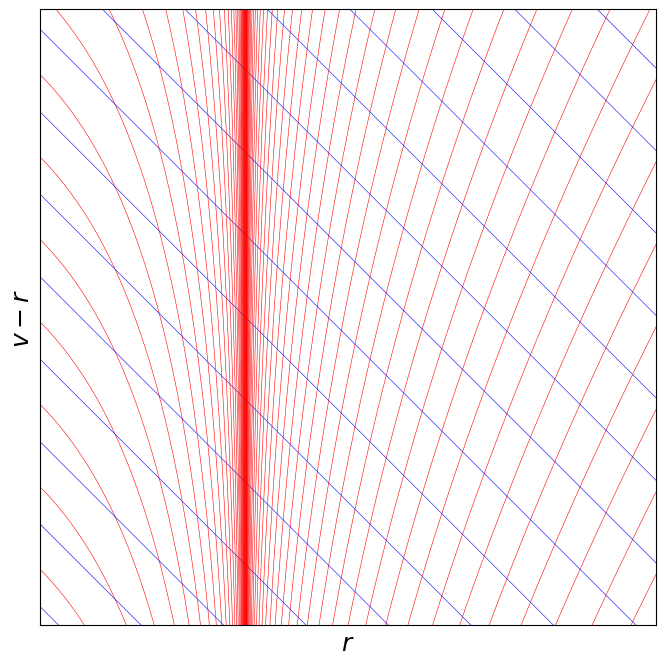
\includegraphics[width=0.48\textwidth]{EF-null.png}
    \caption{
        Null structure near the Schwarzschild event horizon in ingoing Eddington--Finkelstein coordinates $(v,r)$. Outgoing null rays (red) and ingoing null rays (blue) are shown. The vertical line at $r=r_h$ represents a null generator of $\mathcal{H}^+$. Its apparent ``length'' in the diagram encodes the causal \emph{order} of distinct events, not metrical duration: all points along the generator occur at the same areal radius $r_h$, hence at zero invariant spatial separation, and by Theorem~\ref{thm:metric-singularity} at zero temporal separation as well. Distinct horizon-crossing events correspond to distinct manifold points but are metrically coincident; the vertical extent depicted here therefore does \emph{not} represent metrical duration or physical extent in the Lorentzian geometry.
    }
    \label{fig:EF-null}
\end{figure}

The same fact appears in the line element directly, and it appears \emph{forced}---in any chart at all. Take any coordinates $(t,r,\theta,\phi)$ in which $r$ is the areal radius, and follow a generator of $\mathcal{H}^+$. Along it the areal radius is constant and the angle is fixed, $dr=d\theta=d\phi=0$, so every term of the line element carrying a $dr$ or an angular increment drops, and the interval reduces to
\[
ds^2 = g_{tt}\,dt^2 .
\]
The generator is null, so $ds^2=0$; and $dt\neq0$, because once $dr$ and the angles are held fixed the time coordinate is the only direction left for the curve to advance along. A nonzero $dt^2$, multiplied by $g_{tt}$, is required to equal zero: the time coefficient is left alone in an equation that demands zero, with nowhere to go. Hence $g_{tt}=0$. No component of the metric was specified anywhere in this argument; the conclusion is therefore not a fact checked chart by chart but one \emph{forced in every chart}, the null condition annihilating the time coefficient the instant the spatial increments vanish. This is the entire content of the phrase ``any way the geometry is sliced'': not that some privileged slicing makes the events simultaneous, but that no slicing can fail to, the algebra leaving the coefficient no alternative. The coordinate increment $dt$ between two events on a generator may itself be finite and nonzero---in a horizon-penetrating chart it is---and that finite increment is precisely the quantity the metric multiplies by zero. It is the input that forces the collapse, not an escape from it.

In ingoing Eddington--Finkelstein coordinates~\cite{Finkelstein1958,MTW1973} the surviving coefficient is the lapse factor $g_{vv}=-(1-r_h/r)$, which vanishes at $r=r_h$; the apparent vertical extent of the generator in such a diagram (Fig.~\ref{fig:EF-null}) is this vanishing coefficient multiplying a nonzero $dv$---causal \emph{order} drawn as coordinate length, carrying no metrical duration. The geometric argument by Theorem~\ref{thm:metric-singularity} and this algebraic forcing are two readings of one structure: along each generator of $\mathcal{H}^+$ the horizon-crossing events occur at once---radially, temporally, and spatiotemporally---in every chart. The horizon is the 2-sphere of such generators, each a distinct direction of approach. Two events on different generators are spacelike-separated across that sphere---but they are not events the theorem relates: they fail hypothesis~(a), and every horizon-crossing event lies on a single generator. The angular separation is therefore neither a residual extent left uncollapsed nor a sector in which the result is weaker; it is not what the metric singularity is. Along every generator the collapse is total, and that is the entire content of the horizon's metric-singular structure.

\begin{remark}[The forcing in a horizon-penetrating chart]
It is worth running the argument in the chart most often used to show that nothing singular happens at the horizon. In Painlev\'e--Gullstrand coordinates $(T,r,\theta,\phi)$ the metric is regular across $r=r_h$ and the slices $T=\mathrm{const}$ are spacelike and penetrate the horizon, so that two events on a single generator sit at the same $r_h$ but at \emph{distinct, finite} Painlev\'e times, $\Delta T\neq0$. Run the same reduction: along the generator $dr=d\theta=d\phi=0$, the cross term $2\sqrt{r_h/r}\,dT\,dr$ dies with $dr$, and the interval is $ds^2=g_{TT}\,dT^2$ with $g_{TT}=-(1-r_h/r)=0$ at $r_h$. The horizon-penetrating chart returns the same verdict: zero metrical separation. The finite $\Delta T$ a reader may invoke as a counterexample is not one; it is the nonzero increment the null condition requires the coefficient to annihilate---the hypothesis of the argument, not a refutation of it. The more sharply a slicing insists that the generator has a finite time-extent, the more directly it exhibits $g_{TT}\to0$.
\end{remark}

It is worth saying what the vanishing coefficient is, invariantly, for it is not chart-dependent. In coordinates adapted to the static symmetry it is $g_{tt}=g(\zeta,\zeta)$, the squared norm of the timelike Killing vector $\zeta=\partial_t$; its vanishing at $r_h$ is the Killing-horizon condition $|\zeta|^2=0$, a scalar, and on the Killing horizon $\zeta$ is null and tangent to the generators. A scalar carries no slicing to be tested against: $|\zeta|^2=0$ is the invariant of which ``$g_{tt}=0$ in this chart'' is merely the reading. The areal-radius gradient tells the same story---$|\nabla r|^2=g^{ab}\,\partial_a r\,\partial_b r=g^{rr}$ vanishes at $r_h$, so the direction spacelike in the exterior degenerates onto the null generator, leaving no spacelike radial direction at the horizon to carry a separation. The two invariant separations the geometry supplies between two events on a generator therefore both vanish: the interval $\Delta s^2=0$ (null) and the areal-radius separation $\Delta r=0$ (an invariant scalar, constant along the generator).\rcpt{P01_metric_singularity_algebra} This is the statement the infinite-redshift and Killing-horizon notions, read from the same factor, do not make. Each of those is a property holding \emph{at} the surface---a redshift diverging, a Killing field gone null---compatible with reading the horizon as an extended null hypersurface persisting through time. The metric singularity is the relation \emph{between} distinct events on a generator: null-separated, sharing the areal radius, and assigned no metrical separation of any kind.

\begin{corollary}[Degeneracy of Horizon-Crossing Events in EF Coordinates]
In Schwarzschild spacetime expressed in ingoing Eddington--Finkelstein coordinates $(v,r)$, let $\mathcal{H}^{+}$ denote the future event horizon $r=r_h$~\cite{Hawking1973}, and let $p$ and $q$ be two distinct horizon-crossing events lying on the same null generator of $\mathcal{H}^{+}$, with $q$ to the future of $p$ along the generator.

For an exterior observer at fixed areal radius $r>r_h$, the events $p$ and $q$ lie on distinct points of the null boundary of the observer's causal past, and are therefore causally ordered but null-related. Because both occur at $r=r_h$, they are spatially coincident in the sense of Theorem~\ref{thm:metric-singularity}(b); the theorem therefore applies, and $p$ and $q$ are metrically coincident. An exterior observer can assign them no invariant temporal separation: all such events occur at the same location $r=r_h$ and admit no metrical duration between them.

Thus the apparent ``vertical separation'' of horizon points in an Eddington--Finkelstein diagram, as in Fig.~\ref{fig:EF-null}, reflects only the causal ordering of distinct manifold events. It does not encode any geometric or physical temporal distance.
\end{corollary}

Having established that $\mathcal{H}^+$ is a metric singularity, we now turn to the causal structure of gravitational collapse and black-hole mergers, where the geometry of null boundaries determines the portion of the collapsing worldtube that can influence events in the external universe.

\section{Application: gravitational collapse and black hole merger causality}\label{sec:4}

The causal structure of gravitational collapse, event horizon occurrence, and black hole mergers is most transparently described in the Schwarzschild geometry, with hypothetical processes modeled through purely radial motion. The forcing of Section~\ref{sec:3} is not special to Schwarzschild; it holds at any Killing horizon. The horizon generators are the orbits of the horizon-generating Killing field $\chi$---for Schwarzschild $\chi=\zeta=\partial_t$, for Kerr $\chi=\partial_t+\Omega_H\,\partial_\phi$ with $\Omega_H$ the angular velocity of the horizon---which is null there, $|\chi|^2=0$. Passing to coordinates adapted to $\chi$ (co-rotating, in the Kerr case), a generator advances in the $\chi$-time alone, at fixed values of the remaining coordinates; the line element along it reduces to $ds^2=|\chi|^2\,d\tau^2$, the generator is null, $d\tau\neq0$, and $|\chi|^2=0$ is forced exactly as before. Two events on a generator are therefore null-separated; and because the generator is a single integral curve of the invariantly-defined field $\chi$, at fixed values of $r$ and $\theta$, the two share an invariant spatial location---lying on one orbit of $\chi$ \emph{is} the spatial coincidence that hypothesis~(b) requires, the co-rotating chart only the frame in which it reads as a fixed spatial coordinate. The metric therefore assigns them no separation, and the Kerr event horizon is a metric singularity by the same argument. The Schwarzschild presentation in terms of the areal radius over the round symmetry spheres is the non-rotating specialization---$\Omega_H=0$, $\chi=\partial_t$, generators that do not twist, forced coefficient $g_{tt}=|\zeta|^2$; the static lone-survivor reduction fails for Kerr only because the generator twists in the static azimuth and $g_{tt}$ there is nonzero (its vanishing locus is the ergosphere, lying outside the horizon except at the poles), not because the structure fails to carry over. For clarity of exposition, and because the radial collapse and merger construction of this section is carried out only in this case, we restrict attention to Schwarzschild spacetime.

Figure~\ref{fig:collapse-infall} illustrates a standard radial collapse scenario~\cite{Oppenheimer1939b,Penrose1965} in ingoing Eddington--Finkelstein coordinates. The surface of the collapsing star follows a timelike worldline and crosses $r_h$ in finite proper time, later forming a curvature singularity at $r=0$. An external observer remains at fixed areal radius $r>r_h$ just beyond the star's original radius, and releases two test masses toward the collapsing object at different proper times. Test mass~1 intersects the stellar surface before the formation of the horizon, while Test mass~2 is released sufficiently late that its ingoing null ray at the moment of release fails to intersect the worldline of the collapsing surface at $r>r_h$.

\begin{figure}[t]
    \centering
    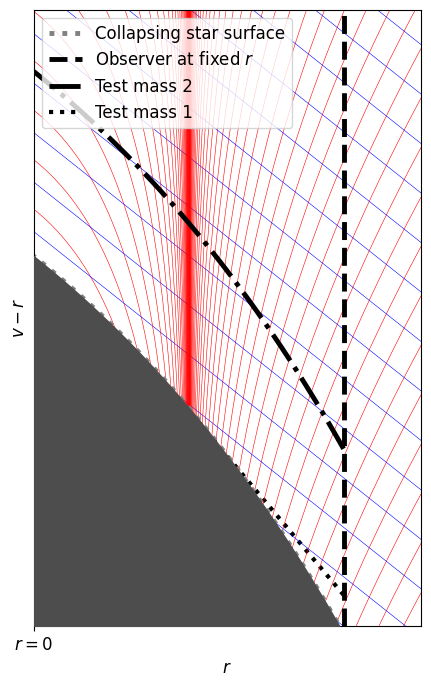
\includegraphics[width=0.48\textwidth]{collapse-infall.png}
    \caption{Radial gravitational collapse in ingoing Eddington--Finkelstein coordinates. The dotted grey curve represents the collapsing star's surface. The dashed curve is an external observer held at fixed radius $r>r_h$. Test mass~1 (dotted) reaches the stellar surface prior to horizon formation. Test mass~2 (dash--dot) is released later, and its ingoing null signal (blue grid) no longer intersects the collapsing surface. Outgoing null rays (red grid) emitted in the exterior region reach the observer, who therefore only ever sees the star and infalling masses asymptotically approach $r_h$. The shaded region indicates the stellar interior.}
    \label{fig:collapse-infall}
\end{figure}

Outgoing null rays in the exterior region, shown in red, all intersect the observer's worldline. Thus, regardless of how long the observer waits, the collapsing surface is never seen to reach $r_h$, since all (null-related) horizon events are spacelike separated from any finite-time exterior event. Even if the observer were equipped with an antenna capable of detecting signals of arbitrary wavelength, the portion of the stellar surface visible to them would only approach $r_h$ as their own proper time tends to infinity.

Before turning to the behavior of the test masses and the application of the theorem and its corollary, it is helpful to summarize the observational appearance of mergers from the standpoint of such an exterior observer, at fixed $r>r_h$. If the observer is equipped with a perfect antenna and gravitational wave detector, they will continually see the collapsing surface at radii strictly larger than $r_h$. Therefore, any merger event that generates gravitational waves the observer later sees must have occurred at a time when the stellar surface remained visible in their causal past. Consequently, at the moment the merger signal arrives, the observer sees a consistent picture: the collapsing mass continues to asymptotically approach $r_h$, a test mass or additional object falls radially inward and meets it, a burst of gravitational radiation is emitted and later detected, and a post-merger object is subsequently observed to continue its approach toward a new effective radius $r'_h$ determined by the total mass. Since the merger event lies within the observer's causal past, and since its outcome remains visible afterward, the entire process \textit{must} have occurred in the region of the spacetime where both bodies remained larger than their respective horizon radii.

\begin{remark}
It is common in the literature, going back to the defining papers~\cite{hawking1971,Penrose1969}, to refer to compact objects that will develop event horizons as ``collapsed objects''---in the past tense, as completed structures, even in contexts where the horizon-formation event has not yet occurred relative to any finite exterior time. The verb tense is doing unstated work: it presupposes that the horizon-formation event is in the causal past of an exterior observer. Hawking's own causal definition of the event horizon as $\mathcal{H}^+ = \partial J^-(\mathcal{I}^+)$ makes clear that such a horizon is a null future boundary, not a structure occurring at any finite exterior time. The two usages cannot be conflated; that they have been, repeatedly and in the foundational literature, is the linguistic seam this paper is correcting.

Just as referring to M31~V1 as a ``supernova remnant'' would implicitly place its supernova event in our causal past, Hawking's informal use of ``collapsed object'' implicitly places the horizon-formation event in the past of an exterior observer (whether the gravitational-wave generation event or our later observation of it)---a usage that contrasts with his own causal definition of the event horizon. The present paper's task, at its core, is to retire that usage: in standard general relativity, no collapsed object occurs on any finite exterior-time slice---there are only objects asymptotically approaching the metric-singularity structure of their horizons in the infinite exterior-time limit. The grammar must follow the geometry.
\end{remark}

\begin{remark}
It is sometimes informally stated that gravitational waves detected in the external universe arise from mergers that have already passed their respective horizon-formation events~\cite{abbott2016}. Within the causal framework developed above, such a description is incompatible with the structure of null boundaries. The horizon-formation event for a collapsing object never lies within the past light cone of any gravitational-wave generation event that is itself visible to an exterior observer. Since gravitational fields, light signals, and gravitational waves all propagate along null geodesics, no event outside an emission event’s causal past can influence its generation. The situation is directly analogous to the M31~V1 example: we do not now observe its supernova remnant because that event does not lie within our causal past. Similarly, any gravitational-wave generation event accessible to an exterior observer must lie in a region where the relevant mass distributions were still larger than their horizon radii in the causal sense established above.
\end{remark}

Having laid this conceptual groundwork, we can now proceed to interpret the causal generation of gravitational waves in the scenario shown in Figure~\ref{fig:collapse-infall}, in the case of the two test-mass collisions.

Since test mass 1 encounters the collapsing surface while its radius is clearly larger than $r_h$, the interpretation is trivial. The wave generation occurs when the two masses are sufficiently close that the waves are generated in the strong field exterior. Those gravitational waves subsequently travel along an outgoing null line and are later observed by the observer at fixed $r$.

The case of test mass 2 is far more interesting and informative, and highlights the metrical degeneracy in the horizon vicinity remarkably well. Note that as the test mass approaches $r_h$, the most recent causal signal along the null connection to the collapsing star comes from ever closer in $r$. The situation is exactly the ``shrinking Andromeda'' limit of Section~\ref{sec:1}: the radial separation across the null connection contracts toward zero, so the emission and observation events approach spatial coincidence, and by Theorem~\ref{thm:metric-singularity} their temporal separation collapses with it. One is tempted to interpret the graphical separation of these two events in Figure~\ref{fig:collapse-infall} as implying temporal distance, but the metric-singularity structure of the horizon events ensures this is merely an artifact of the chosen coordinate system, which separates them by causal, not metrical, order. Thus the figure, accurately interpreted, illustrates that the distance in $r$ between the collapsing star's surface and the test mass continually decreases when measured across their null connection. And if gravitational waves are generated, and later seen by the external observer, the wave generation event must have occurred at causal times preceding the horizon-formation event along both worldlines, relative to their shared null connection.

\section{Asymptotic alignment of exterior temporal slicings with the horizon}\label{sec:5}
The event horizon $\mathcal{H}^+=\partial J^-(\mathscr{I}^+)$ is the null future boundary of the exterior domain: every one of its generators is a limit of the past-light-cone boundaries of exterior observers. Any Cauchy temporal function of the exterior must therefore accommodate this boundary---as one moves to increasingly late exterior times, the observer's level sets are forced to approach and ultimately ``pile up'' against $\mathcal{H}^+$, meeting it only in the limit of infinite exterior time. This accumulation is a consequence of causal structure alone, independent of the metric-singularity identification of Sections~\ref{sec:2}--\ref{sec:3}; we record it first in full generality.

\begin{proposition}[Asymptotic exterior slicings of a future event horizon]\label{prop:causal-alignment}
Let $(M,g)$ be any asymptotically flat, globally hyperbolic spacetime with future event horizon $\mathcal{H}^+=\partial J^-(\mathscr{I}^+)$, let $O$ be a future-complete worldline in the exterior domain---one that persists to future infinity, with $O(\tau)\to i^+$ as $\tau\to\infty$---and let $\Theta:M\to\mathbb{R}$ be any smooth Cauchy temporal function of the exterior adapted to $O$, meaning $\Theta(O(\tau))=\tau+\mathrm{const}$. Then the past-light-cone cross-sections $\partial J^-(O(\tau))\cap\mathcal{H}^+$ rise toward future infinity along $\mathcal{H}^+$ as $\tau\to\infty$; the level sets $S_\tau$ accumulate on $\mathcal{H}^+$, their tangent hyperplanes becoming asymptotically tangent to its generators in direction; and each finite-$\Theta$ slice lies entirely in the exterior region, meeting $\mathcal{H}^+$ only in the limit. Consequently the event horizon does not occur on any finite exterior time-slice: it occurs only as the null future boundary approached in the infinite-time limit.
\end{proposition}

\begin{proof}
By global hyperbolicity, each level set $S_\tau$ meets the past light cone $J^-(O(\tau))$ in a smooth spacelike hypersurface, and $\partial J^-(O(\tau))$ is a null hypersurface. Because $O$ is future-complete with $O(\tau)\to i^+$, its past light cones exhaust the causal past of future null infinity as $\tau\to\infty$; by the defining property of the event horizon, $\mathcal{H}^+=\partial J^-(\mathscr{I}^+)$, every generator of $\mathcal{H}^+$ is then a limit of the past-light-cone boundaries $\partial J^-(O(\tau))$~\cite{hawking1971,Wald1984}, which therefore approach $\mathcal{H}^+$ monotonically as $\tau\to\infty$, so their cross-sections with $\mathcal{H}^+$ rise toward future infinity and the slices $S_\tau$ accumulate on it, their tangent spaces becoming asymptotically tangent to the generators. Because $\mathcal{H}^+$ is the future boundary of the exterior domain, no finite-$\Theta$ slice crosses it; tangency is attained only in the limit $\tau\to\infty$. The argument invokes only global hyperbolicity, the defining property of the horizon, and the future-completeness of $O$, and so holds for the event horizon of any asymptotically flat, globally hyperbolic spacetime.
\end{proof}

In the Schwarzschild geometry this degeneration can be exhibited explicitly, and the metric-singularity structure of $\mathcal{H}^+$ established in Sections~\ref{sec:2}--\ref{sec:3} additionally fixes its \emph{magnitude}---the rate at which the lapse of the foliation collapses---which Proposition~\ref{prop:causal-alignment} leaves open.

\begin{lemma}[Asymptotic Alignment of Exterior Temporal Slicings]\label{lem:alignment}
Let $(M,g)$ be the exterior region of the Schwarzschild spacetime with areal radius $r>r_h$, and let
\[O : \tau \mapsto \bigl(v(\tau),\, r_0\bigr)\]
be an observer at fixed radius $r_0>r_h$, parametrized by proper time $\tau$.  
Let $\Theta : M \to \mathbb{R}$ be any smooth Cauchy temporal function~\cite{BernalSanchez2005} of $(M,g)$ adapted to $O$, meaning
\[\Theta\bigl(O(\tau)\bigr)=\tau+\mathrm{const}.\]
For each $\tau$, define the level set 
\[S_\tau := \{\, x \in M : \Theta(x)=\tau\,\}.\]

Then:
\begin{enumerate}

\item[(i)] \textbf{(Accumulation on the horizon)}  
The past-light-cone cross-sections $\partial J^{-}(O(\tau)) \cap \mathcal{H}^+$ rise toward future infinity along $\mathcal{H}^+$ as $\tau \to \infty$, and the slices $S_\tau$ accumulate on $\mathcal{H}^+$. In the angle-suppressed radial picture of Fig.~\ref{fig:stationary-t-on-EF}, where $\mathcal{H}^+$ appears as one generator, this cross-section is the single point at the observer's angular position climbing that generator.

\item[(ii)] \textbf{(Asymptotic alignment)}  
As $S_\tau$ accumulates on $\mathcal{H}^+$, the tangent hyperplanes of $S_\tau$ become asymptotically tangent to the generator and the lapse of the foliation collapses,
\begin{eqnarray*}
    &&g^{ab}(\nabla_a \Theta)(\nabla_b \Theta)\,\longrightarrow\,-\infty\\
    &&\text{along } \partial J^{-}(O(\tau)) \cap \mathcal{H}^+ 
\quad\text{as } \tau\to\infty.
\end{eqnarray*}
Thus $\nabla\Theta$ aligns with the generator in direction while its norm diverges---equivalently, the lapse $N\to0$---and $S_\tau$ meets $\mathcal{H}^+$ only in the limit.

\end{enumerate}
\end{lemma}

\begin{figure}[t]
\centering
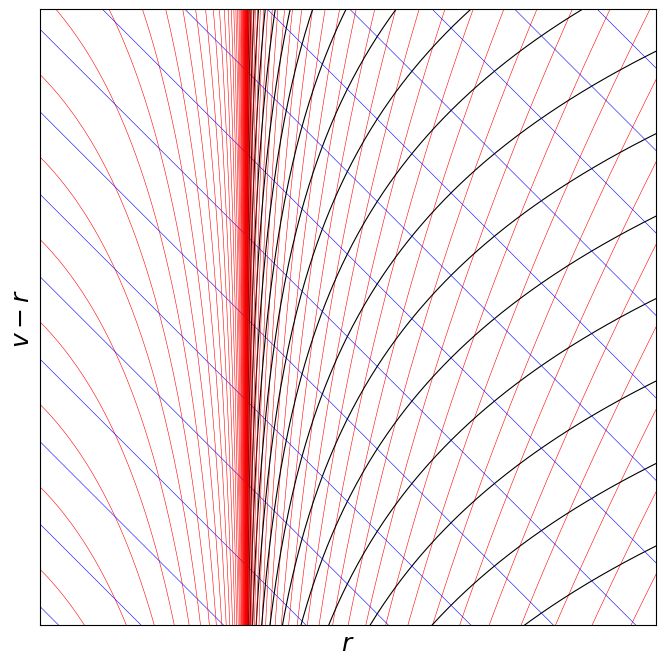
\includegraphics[width=0.48\textwidth]{stationary-t-on-EF.png}
\caption{
Level sets of the stationary Schwarzschild time coordinate $t$ (black) plotted on an ingoing Eddington--Finkelstein diagram. Outgoing (red) and ingoing (blue) null rays are shown. The Schwarzschild slices $t=\mathrm{const}$ tilt upward and accumulate along a single generator of $\mathcal{H}^+$, becoming asymptotically tangent to it. Although this image uses the stationary $t$ coordinate, the asymptotic piling-up is generic: the accumulation and directional alignment follow from the horizon's causal structure (Proposition~\ref{prop:causal-alignment}), and in Schwarzschild the degeneration is realized explicitly by Lemma~\ref{lem:alignment}, so any Cauchy temporal function of the exterior must degenerate in this way, with all late-time slicings converging on $\mathcal{H}^+$.
}
\label{fig:stationary-t-on-EF}
\end{figure}

\begin{proof}
For each $\tau$, the level set $S_\tau$ intersects the past light cone $J^{-}(O(\tau))$ in a smooth spacelike hypersurface.  
Since the Schwarzschild exterior is globally hyperbolic~\cite{Wald1984}, the boundary $\partial J^{-}(O(\tau))$ is a smooth null hypersurface meeting $\mathcal{H}^+$ in a cross-section that rises toward the future as $\tau\to\infty$ (a single point on the observer's radial generator in the angle-suppressed picture).

As $\tau\to\infty$, the sets $\partial J^{-}(O(\tau))$ monotonically approach $\mathcal{H}^+$, and by the defining property of the event horizon~\cite{hawking1971}, every generator of $\mathcal{H}^+$ is the limit of such past-light-cone boundaries.  
Thus the cross-sections $\partial J^{-}(O(\tau))\cap\mathcal{H}^+$ rise along $\mathcal{H}^+$ and $S_\tau$ accumulates on it, establishing (i).

Since $S_\tau$ intersects $\partial J^{-}(O(\tau))$ transversely and $\partial J^{-}(O(\tau))$ approaches a null hypersurface, the tangent spaces $T(S_\tau)$ become asymptotically tangent to $\mathcal{H}^+$ along $\partial J^{-}(O(\tau))\cap\mathcal{H}^+$. This fixes the \emph{direction} of $\nabla\Theta$: it aligns with the generator and becomes asymptotically null.

The \emph{magnitude} is fixed separately, by the adaptation condition. Tangency alone is compatible with either $g^{ab}(\nabla_a\Theta)(\nabla_b\Theta)\to 0^-$ or $\to-\infty$; the sign is settled not by the tilt but by the requirement $\Theta(O(\tau))=\tau+\mathrm{const}$, which fixes the increment of $\Theta$ between successive slices at the observer's worldline. Because the slices accumulate on $\mathcal{H}^+$ by~(i) while the redshift factor relating the adapted time to proper time vanishes there ($-g_{tt}\to0$ as $r\to r_h$ in the stationary chart, equivalently the lapse $N\to0$), a fixed $\Theta$-increment must be realized over a vanishing lapse: $\Theta$ changes by a finite amount across proper-time intervals shrinking to zero, so $|\nabla\Theta|\to\infty$. Hence $g^{ab}(\nabla_a\Theta)(\nabla_b\Theta)\to-\infty$ and the lapse $N=|\,g^{ab}(\nabla_a\Theta)(\nabla_b\Theta)\,|^{-1/2}\to 0$. For the stationary slicing this is explicit---$g^{ab}(\nabla_a t)(\nabla_b t)=g^{tt}=-1/(1-r_h/r)\to-\infty$, $N=\sqrt{1-r_h/r}\to 0$---and the argument above shows the same collapse holds for any Cauchy temporal function of the exterior adapted to $O$, giving (ii).
\end{proof}

\begin{remark}
As Proposition~\ref{prop:causal-alignment} records, the accumulation~(i), the directional alignment of $\nabla\Theta$, and the conclusion that the horizon does not occur at any finite exterior time use only the global hyperbolicity of the exterior and the defining property $\mathcal{H}^+=\partial J^-(\mathscr{I}^+)$; they appeal to no Schwarzschild-specific feature. The \emph{magnitude} half of~(ii)---the lapse collapse $N\to0$---rests on more than this causal structure: it turns on the vanishing of the redshift factor $-g_{tt}\to0$ at the horizon, a metric fact. This is a general feature of a Killing (or, more broadly, causal) horizon and is not special to Schwarzschild; but it is a metric input, not a consequence of causal structure alone, and the identification of $\mathcal{H}^+$ as a metric singularity in Section~\ref{sec:3} (which in the spherically symmetric case requires only the constancy of the areal radius along the generator, and which Section~\ref{sec:4} extends to any Killing horizon through the vanishing $|\chi|^2=0$ of the horizon-generating field) is the second such metric step, not, as a stronger reading might suppose, the only one.
\end{remark}

\begin{remark}
For any exterior observer---and, more generally, at all points in the exterior region $r>r_h$---the event horizon $\mathcal{H}^+$ lies permanently at the null future boundary of the observer's causal future. In particular, if $\Theta$ is any Cauchy temporal function of the exterior adapted to such an observer, then each finite-$\Theta$ slice $S_\Theta$ lies entirely in the region $r>r_h$ and therefore never intersects $\mathcal{H}^+$ (e.g.~Figure~\ref{fig:stationary-t-on-EF}). Only in the limit $\Theta \to +\infty$ do the slices approach and become tangent to $\mathcal{H}^+$.

Thus, relative to any admissible exterior time coordinate, the event horizon does not occur at any finite time within the exterior domain. Within the causal domain of the external universe, the event horizon does not ``exist'' as a present structure---that is, it is not present across any sequence of finite exterior time-slices adapted to an exterior observer. Rather, it \textit{occurs} only as the null future boundary approached in the infinite-time limit: a singular occurrence at the end of the universe. This conclusion concerns only the behavior of exterior-adapted slicings and does not address the global structure of the spacetime beyond that domain.
\end{remark}

\begin{remark}
It is important to emphasize that Lemma~\ref{lem:alignment} is not a statement about observational limitations or about the causal past of any particular observer. Rather, it characterises the structure of every temporal slice $S_\Theta$ adapted to any exterior worldline. Such slices extend well beyond the observer's past light cone and include all events that may be taken as ``out there now'' relative to that observer, yet none of them---for any finite value of $\Theta$---ever intersect the event horizon or contain any portion of a future singularity. Each finite-$\Theta$ slice contains only still-collapsing matter. The event horizon therefore does not occur as part of any finite exterior time-slice; it occurs only once, at the infinite-time boundary of the exterior domain. In maximal extensions, the apparent vertical ``stack'' of horizon points merely displays the causal ordering of distinct manifold events that are nevertheless metrically coincident, rather than a temporal extension of the horizon within finite exterior time.
\end{remark}

\section{The standard problems of black-hole physics}\label{sec:problems}
The result of \S\ref{sec:5}---that within the causal domain of the external universe the event horizon occurs only as the null future boundary, present on no finite exterior slice and approached only in the infinite-time limit---bears on a family of problems that have organised black-hole physics for half a century. Each of them presupposes a physically realised, globally completed event horizon: a surface that has formed, that separates a causally disconnected interior, and that persists as a structure of the spacetime. That presupposition is what the preceding sections deny for any black hole causally accessible to the external universe. We draw the consequences using only the standard causal structure the rest of the paper uses, and no modification of general relativity. Drawn here on causal structure alone, these dissolutions do not stand in isolation: gathered with the framework's others and weighed as theory-choice---dissolution by identity, not management by conjecture---they form the first synthesis of the companion framework paper~\cite{JanzenCRframework}, where the same distinction between the evolving existent and its maximally extended representation is shown to dissolve a wider family of general relativity's standing problems at one stroke. That first synthesis is the programme's unification: it reads one maximally symmetric de~Sitter substrate as the common ground of general relativity's solution space, of the discrete $CPT$ and charge-conjugation structure, and of the gauge algebra borne on its conjugate real form~\cite{JanzenCRframework}. The present result---reached, as throughout, from standard general relativity alone---is the structural forcing at the root of that reading: the everywhere-real null boundary on which the substrate's ontology rests~\cite{JanzenGeometricCore}, and, with the empirical cosmology, one of the two tests by which the whole is held to the world rather than to its own coherence~\cite{JanzenCRframework,JanzenShadowExistence}.

It is worth making explicit, on grounds that reinforce \S\ref{sec:5} from the side of the source rather than the observer's slicing, why no completed horizon is realised. The event horizon is a \emph{global} structure: its location is defined only with respect to the entire future development of the spacetime, $\mathcal{H}^+=\partial J^-(\mathscr{I}^+)$. A present astrophysical black hole---one embedded in a universe still forming structure---continues to merge and accrete, and every such interaction is part of the spacetime's dynamical evolution, not fixed future boundary data. At an interaction event $p$, the exterior geometry to the future of the outgoing null hypersurface generated at $p$ must be replaced by the solution carrying the new mass, energy, and angular momentum; the pre-interaction exterior cannot be extended across that hypersurface without describing a counterfactual spacetime in which the interaction never occurred. Because general relativity is local---the exterior geometry is generated causally by the matter worldtube, along outgoing null rays that leave the collapsing surface \emph{before} any horizon, as \S\ref{sec:4} makes explicit for the observed signal---every outgoing generator of the realised exterior traces back to the pre-horizon worldtube, never to a completed horizon or interior. A horizon defined prior to an interaction is thus not the event horizon of the realised spacetime but of an auxiliary solution assuming no further interaction occurs; and since a present black hole always has further mergers and accretion in its future, no such object possesses a globally completed horizon as a physical structure. Its collapse is perpetually asymptotic, the exterior repeatedly regenerated before any horizon forms---the same conclusion \S\ref{sec:5} reaches through the exterior foliations, now read along the source's own generators. The two routes agree.

\subsection*{Trapped surfaces and the singularity theorems}
Penrose's theorem establishes that a closed trapped surface, with the null energy condition and suitable global assumptions, forces geodesic incompleteness---a singularity~\cite{Penrose1965}. Its hypothesis is a \emph{realised} closed trapped surface, an object interior to the event horizon. By the above, no completed horizon, and so no trapped surface it would enclose, is ever physically realised for a black hole causally accessible to the external universe. The theorem is therefore a correct mathematical result whose physical precondition is never met in the astrophysical domain: it describes the auxiliary completed geometry, not the realised spacetime. Singularities are, on this reading, not \emph{avoided} by any new physics or any modification of general relativity---they are rendered \emph{physically irrelevant} by causal structure alone, the curvature singularity of the maximally extended geometry (the infinite-curvature species of the genus of \S\ref{sec:2}--\S\ref{sec:3}, \cite{JanzenCircle}) remaining a feature of a global extension the realised worldtube never instantiates. For the same reason cosmic censorship---the conjecture that realistic collapse keeps its singularities behind horizons---is not a hypothesis the present universe requires: where no singularity is physically realised, none needs to be censored.

\subsection*{Hawking radiation}
The semiclassical derivation of black-hole evaporation~\cite{Hawking1975} evolves a quantum field on a fixed background containing a globally completed horizon and computes a Bogoliubov transformation between the in-vacuum at $\mathscr{I}^-$ and the out-vacuum at $\mathscr{I}^+$; the inequivalence of those vacua is the thermal flux. The construction requires three things: a globally defined horizon; a completed causal structure joining $\mathscr{I}^-$ to $\mathscr{I}^+$ across it; and the permanent loss of causal contact between exterior and interior modes that renders the two vacua inequivalent. \emph{That third requirement has an exact criterion rather than a qualitative one}: two Fock representations are unitarily equivalent precisely when the Bogoliubov coefficient $\beta$ is Hilbert--Schmidt~\cite{Shale1962}, and a thermal $\beta$ fails that test at the infrared end, where its $1/\omega$ tail makes $\lVert\beta\rVert_{\mathrm{HS}}^{2}$ logarithmically divergent. \emph{The criterion supplies the conclusion rather than qualifying it}---the thermal flux \emph{is} that inequivalence---and it is equally what makes the absence of a realised background decisive: a criterion on $\beta$ has nothing to be applied to when there is no $\beta$ to compute\ldg{functional_analysis}. None of the three is realised for a present astrophysical black hole. The field is defined on a single connected exterior domain with no permanently inaccessible region; no generator of that domain is grounded in a completed horizon; and no mode is traced across one. The Bogoliubov transformation that would yield the thermal spectrum therefore has no realised background to be computed on---the mathematical horizon of the auxiliary extension is not part of the physical spacetime and cannot define inequivalent in- and out-vacua.

\emph{One further distinction belongs here, because the companion programme puts a thermal state on a horizon
and a reader holding both results together will want the two reconciled.} The canonical companion closes the
quantization of the layer's scale factor by placing the regular Euclidean---Hartle--Hawking---state at a
horizon of surface gravity $\kappa=1/\alpha$~\cite{JanzenCanonicalTime}. That is not in tension with what is
established here, and the reason is that the two horizons are different objects. The horizon whose thermal
state is denied above is the \emph{collapse} horizon of an astrophysical black hole, and the ground of the
denial is that it is never completed at finite exterior time---there is no realised background on which the
Bogoliubov construction can be carried out. The horizon carrying the Euclidean state there is the
\emph{cosmological} horizon of the substrate: it is not the endpoint of a collapse, requires no completion, and
is realised on every slice. \emph{The argument of this paper turns on a horizon that never finishes forming; it
says nothing against a horizon that was never forming.}

\emph{And there is a third horizon a reader will bring, which is the one that decides what the criterion here
actually is.} A uniformly accelerated observer in flat space, carrying proper acceleration $a$, detects an
exactly thermal spectrum at temperature $a/2\pi$~\cite{Unruh1976}. The horizon responsible is the Rindler
horizon: the bifurcate Killing horizon of the boost field, uncontroversially observer-dependent---a different
accelerated observer has a different one, an inertial observer has none---with no gravity, no collapse, and
nothing anyone would call a completed physical surface in the sense of a black hole's. \emph{The spectrum is
thermal all the same.}

\emph{So an argument of the form ``the horizon is perspectival, therefore there is no thermal flux'' is refuted
before it starts, and that is not the argument made here.} What is denied above is a horizon that is never
\emph{completed}, and completion is a different property from observer-dependence: the Rindler horizon is
observer-dependent and complete---the boost field is an exact Killing field of the whole spacetime and its
horizon is a global structure of that spacetime, available in full without waiting for any future
development. \emph{The two properties come apart precisely at this case, which is why it is the one worth
stating.} Read across the four horizons this programme has occasion to name, the sorting is clean and it is
clean on one criterion only\rcpt{P1_the_unruh_case_is_what_makes_the_criterion_completion_and_not_perspective}: the Rindler horizon (complete, observer-dependent) is thermal; the
substrate's cosmological horizon (complete, observer-dependent) is thermal, and carries the Euclidean state
just discussed; the eternal Schwarzschild horizon (complete, observer-independent) is thermal; and the
collapse horizon of a present astrophysical black hole (never completed) is the one case in which the
Bogoliubov construction has no realised background. \emph{Observer-dependence sorts the first two into the
wrong class; completion sorts all four.}

\emph{On this substrate the accelerated case also says something the flat one cannot, and it is a consequence
of there being a single constant rather than an additional assumption.} In de~Sitter space the accelerated
temperature is $T(a)=\tfrac{1}{2\pi}\sqrt{H^{2}+a^{2}}$~\cite{NarnhoferPeterThirring1996, DeserLevin1997},
which reduces to $a/2\pi$ as $a$ grows and to the Gibbons--Hawking value $H/2\pi$ at rest. Here $H=1/\alpha$
and $\alpha=\sqrt{3/\Lambda}$ is the substrate's only dimensionful constant, so the rest term is exactly the
$\kappa=1/\alpha$ of the Euclidean state above and
\begin{equation}\label{eq:unruh-ds}
T(a)=\frac{1}{2\pi}\sqrt{\frac{1}{\alpha^{2}}+a^{2}}
\end{equation}
carries no adjustable parameter at all: the observer supplies $a$ and the substrate supplies the rest, and
there is nothing else to supply. \emph{The structural difference from the flat statement is that the rest term
does not vanish.} An unaccelerated observer in Minkowski space sees nothing; an unaccelerated observer on this
substrate is already in a thermal state, and acceleration adds to a bath rather than creating one.

\emph{And there is a sharper thing to say about the collapse case, which the framework paper computes for a
different purpose and which has not been set beside this one.} The member a collapse reaches on this
construction is the Nariai one, at which the metric function has a double root and the surface gravity
\emph{vanishes}~\cite{JanzenCRframework}. \emph{So the thermal flux the information paradox requires is absent
twice over and for independent reasons}: absent because no completed horizon is realised, which is this
paper's argument and does not depend on which member is reached; and, granting the completion for the sake of
the objection, $\kappa=0$ at the member that would be completed. \emph{The second is not offered as a
replacement for the first.} A degenerate horizon is the case in which reading a temperature off $\kappa/2\pi$
is least safe---the near-horizon geometry there is the equal-radii $\mathrm{dS}_{2}\times S^{2}$ throat this
programme builds elsewhere~\cite{JanzenCRcosmology}, which carries a scale of its own---and the two readings
are not reconciled here. \emph{What is claimed is the coincidence and not a value}: the configuration at which
the framework says the ringdown carries no scale is the same configuration at which the surface gravity is
zero, and both are the configuration a collapse is said to reach.
\emph{And there is a third thing to say about that configuration, which says what is true of it rather than what cannot be read off it---and the cosmology paper derived it already, for another purpose.} What makes a non-degenerate horizon thermal is not the number $\kappa$ but an exponential: near a simple root $f\sim2\kappa\delta$, so the tortoise coordinate $r_{*}=\int\dd r/f$ is logarithmic, the approach is $\delta\sim e^{2\kappa r_{*}}$, and it is that exponential relation between the affine and Killing parameters that carries a mode's positive frequencies into a Planck spectrum. \emph{At a double root the relation is not available at all}: $f\sim c\,\delta^{2}$ gives $r_{*}\sim-1/c\delta$, a power law, so the construction that produces a thermal spectrum has no first step to take\rcpt{P1_thermality_is_the_exponential_and_a_double_root_has_no_exponential}. \emph{The right statement is therefore not that the temperature is zero but that the mechanism is absent}---and the two are different claims, the first of which this paper has just declined to make. The same $p=1$ against $p=2$ split is what the cosmology paper uses to say what \emph{crosses} the branch point, a non-degenerate horizon's exponential approach imprinting a scale and the degenerate member's power-law approach imprinting none~\cite{JanzenCRcosmology}: one fact serving two purposes, and it was not being read here. \emph{What this does not say is that the configuration is athermal in every sense}---a scale-free power-law approach can still act on a spectrum, which is exactly what the cosmology paper argues it does, and that is a different question from whether a Planck spectrum arises.

\emph{What none of this claims.} It does not claim that Unruh's result is in tension with anything here---the
opposite: it is the case that shows the criterion used above is the one that works. It does not claim a
derivation of the Unruh effect from the substrate, or any new value for a temperature. And it does not claim
that $\kappa=0$ settles the collapse case, which rests on completion and not on a surface gravity.

\emph{And the result of this section does positive work in that construction, which is worth recording because
it is not obvious from either side.} A regular Euclidean state exists at a horizon only if the Euclidean
continuation is smooth there---free of a conical defect, with the curvature finite. That is precisely the
content of the distinction this paper draws: the horizon is a \emph{metric} singularity, at which the spatial
measure collapses while the curvature stays finite, and not a curvature singularity, at which no smooth
Euclidean section would exist and no regular state could be selected. \emph{So the definition supplied here is
what makes the companion's state available}, and through it what makes the imaginary-time segment of the
cosmogenetic contour a well-posed object rather than a formal manoeuvre~\cite{JanzenCRframework,
JanzenCanonicalTime}. The general point is sharper than a single criterion, and worth stating carefully because the obvious
version of it is false. \emph{Finite curvature is sufficient for a continuation to cross a boundary, but it is
not necessary}, and the companion construction crosses two boundaries of opposite type. At this horizon the
curvature is finite while the tortoise measure $r_{*}=\int\dd r/f$ diverges. At the branch point of the
cosmogenetic contour the reverse holds: $f\to-2M/r$ diverges, so \emph{$r_{*}$ converges} while the areal
curvature does not~\cite{JanzenCRframework, JanzenCircle}. Each is crossable, and for opposite reasons---one
because nothing diverges in the geometry, the other because nothing diverges in the measure along which the
crossing is taken. \emph{What the two share is not a property but a negation: neither failure is a failure of
both.} That is worth recording against the habit of reading ``singularity'' as a single verdict; the curvature
criterion and the affine-measure criterion are independent, and this construction realises each without the
other.

The scope of this conclusion is narrower than ``black holes do not radiate,'' and the distinction is essential. What is absent is \emph{horizon-induced} Hawking radiation---the thermal spectrum whose entire mechanism is the completed horizon and the vacuum inequivalence it induces. Local particle-production processes that do \emph{not} require a horizon---strong-field vacuum polarisation and the like---are untouched by the argument and are not excluded; a perpetually collapsing ultra-compact body need not be quiescent. The claim is precisely that the specific mechanism of horizon evaporation has nothing to act on in a spacetime that realises no horizon. It needs no ultraviolet completion of gravity and no modification of quantum theory; it rests on the causal structure already established.

\emph{One standing objection to the standard derivation belongs here too, because this reading has a version of
its own and the scope of what can be said about it is the whole of what is said.} The trans-Planckian problem
observes that the late-time quanta of the Hawking flux, traced backward through the collapse, originate as modes
of arbitrarily high frequency, so that the derivation's output depends on physics above the Planck scale which the
derivation itself does not supply~\cite{Jacobson1991, Unruh1995}. \emph{In that form the objection targets the
Bogoliubov construction, which is not carried out here}---it is an objection to a computation this paper declines
to perform, and it does not transfer as stated. But the reading advanced above has a version that needs no
mode-tracing at all. A static observer at areal radius $r$ outside a still-collapsing surface measures a local
frequency $\omega_{\mathrm{loc}}=\omega_{\infty}/\sqrt{f}$; near a simple root $f\simeq2\kappa\delta$ with
$\delta=r-r_{h}$, so the blueshift factor goes as $\delta^{-1/2}$ and \emph{diverges only as the surface is
reached}. Section~\ref{sec:5} is precisely the statement that it is not reached at any finite exterior time.
\emph{So the blueshift is finite at every finite exterior time, and the divergence sits inside a limit this paper
says is never taken.}

\emph{And the scoping of that is its content, because the available claim is weaker than the one it
resembles---it is not that the blueshift is bounded.} For a radially infalling surface with unit energy per unit
mass, $\dd r/\dd t=-f\sqrt{r_{h}/r}\simeq-2\kappa\delta$ near the root, so $\delta\propto e^{-2\kappa t}$ and
$\omega_{\mathrm{loc}}/\omega_{\infty}\propto e^{\kappa t}$: the factor grows without bound, and its supremum over
exterior time is infinite. \emph{What is available is ``finite at each finite exterior time'' and not
``bounded''}, and the two are not interchangeable here, because the growth is exponential with the same $\kappa$
the preceding paragraph identified as the mechanism of thermality---one exponential seen twice, once as what
carries a mode's positive frequencies into a Planck spectrum and once as what carries the collapsing surface into
the ultraviolet. Taking $\omega_{\infty}\sim\kappa$, the exterior time at which the local frequency first reaches
the Planck value is $\kappa^{-1}\ln(\kappa^{-1}/t_{P})$, the logarithm suppressing nothing: about $2\times10^{-3}$
seconds at a solar mass, $2\times10^{-2}$ seconds at ten, and of order months for the heaviest resolved
supermassive hole\rcpt{P1_the_transplanckian_claim_is_finite_at_each_finite_time_and_it_is_not_bounded}.
\emph{The finiteness is therefore not a suppression of ultraviolet physics but a statement about which limit is
taken}, and the regime is entered on a timescale short by every astrophysical measure.

\emph{What that does and does not buy is worth stating flatly, because the weaker claim is easily read as the
stronger one.} The argument of this section is causal: it turns on the absence of a completed horizon and hence
of a realised background, computes no mode functions, and does not depend on any local frequency being finite.
The sentence above---that the conclusion needs no ultraviolet completion of gravity---is accordingly a claim about
what \emph{the argument} requires, and not a claim that the late-time collapsing surface is free of ultraviolet
physics. \emph{It is not, and this paper does not say it is.} Whether that regime is benign, and what a treatment
of it would have to supply, is not settled here and is not claimed; the companion programme's crossing of the
branch point is where the question has its home~\cite{JanzenCRcosmology, JanzenDynamics}. What is claimed is the
pair: the objection as usually posed is an objection to a construction not performed here, and the corresponding
statement about the realised surface holds \emph{at each finite exterior time and not uniformly}.

\subsection*{The information paradox}
The information-loss paradox arises only if a completed horizon forms and subsequently evaporates, so that quantum evolution must be defined on a spacetime containing a permanently inaccessible interior into which information has fallen and from which only thermal radiation returns. Both premises fail, and together. No completed horizon forms, by the above; and with no horizon-induced radiation there is no evaporation to carry the loss. The realised spacetime remains globally connected: its domain of quantum evolution admits a global Cauchy surface, there is no hidden interior sector to trace over, and unitary evolution is unobstructed. The paradox is therefore not \emph{resolved} by some mechanism that recovers the information---it does not arise, because the spacetime it requires is never physically instantiated. Approaches that would restore unitarity by modifying the near-horizon state while retaining the completed-horizon background~\cite{Vachaspati2007} address a configuration the realised universe does not contain; the present result removes the premise rather than adjusting the response to it.

\subsection*{The laws of black-hole mechanics}
The laws of black-hole mechanics---the constancy of the surface gravity over the horizon, the first law $dM=\tfrac{\kappa}{8\pi}\,dA+\Omega\,dJ+\Phi\,dQ$, and the area theorem that the horizon area never decreases~\cite{Bardeen1973,hawking1971}---are, like Penrose's theorem, correct results whose object is a \emph{realised} event horizon: a null boundary carrying a definite area and surface gravity. That object is, by the above, never instantiated on a finite exterior slice; the horizon occurs only as the metric singularity of the infinite-time boundary, and no finite slice carries the area whose monotonicity the theorem asserts. The laws therefore characterise the auxiliary completed geometry, not the realised worldtube---the classical, area-side companions of the horizon-induced Hawking temperature already set aside above. The Bekenstein--Hawking entropy~\cite{Bekenstein1973}, in the reading on which it is the entropy \emph{of} that horizon, shares their status; what content survives for a perpetually collapsing ultra-compact body---as with the local particle-production processes---is not settled by this argument; what the collapse does produce---its continuation as an expanding cosmology---is the subject of the companion framework and cosmology papers~\cite{JanzenCRframework,JanzenCRcosmology}. The point is only that the specific horizon-thermodynamic apparatus, area law and entropy alike, has on a finite exterior slice no realised horizon to be defined on, exactly as its temperature has none.

\begin{remark}[Consequences for finite-time densities and the programme]
Because the event horizon occurs, for every exterior observer, only as a metric singularity at the infinite-time null boundary, no finite exterior-time slice contains a horizon or the curvature singularity it would enclose. The densities associated with the central singularity therefore never form at any finite exterior time; mass remains finite in extent on every finite slice, with each infalling element asymptotically approaching its own horizon event. This places the present geometric result within a wider programme. The companion slicing construction for the Schwarzschild--de~Sitter family identifies the metric singularity established here as the geometric cause of the horizon-versus-centre asymmetry of the standard description~\cite{JanzenSlicing}; the existence/occurrence distinction this paper turns on---that the horizon \emph{occurs} without ever \emph{existing} on a finite exterior slice---is, there, the same distinction set at the root of the cosmological ontology, where the enduring cosmic time that existence requires is itself empirically forced~\cite{JanzenModernParallax}, the present paper reaching it from standard general relativity alone. That same construction shows the collapse does not end at the centre: the areal radius is signed, and the slicing closes through the locus the chart labels $r=0$---a branch point and not a barrier, the substrate $C^{\infty}$ across it and the curvature divergence there a perspectival artefact of the areal coordinate---continuing onto the real conjugate branch~\cite{JanzenSlicing,JanzenCircle}. Read forward as physics, that branch is an expanding universe: the collapse whose densities never form at finite exterior time continues, past the branch point---finite in the substrate's curvature, the areal divergence belonging to the chart---and out through the seam this paper proves a metric singularity, as the expansion leg of one closed \emph{cosmogenetic bead}, established as a theorem of the construction~\cite{JanzenCRframework}---the seam the single locus collapse and cosmology share, and the progenitor, in the signed-radius geometry, an antimatter black hole~\cite{JanzenCRframework}, whose thermal history the companion cosmogenesis paper reads in the primordial light-element abundances~\cite{JanzenCosmogenesis}. The present paper reaches only the metric-singularity structure, from standard general relativity; the continuation is the companions', established there and theirs to carry. What that continuation leaves genuinely open is the \emph{matter} dynamics of the crossing---the worldline-and-field transition by which matter and observers pass through the shared layer. Its specific home is the companion cosmology, which owns the seam~\cite{JanzenCRcosmology}; a first concrete matter model is carried in the cosmogenesis paper~\cite{JanzenCosmogenesis}; and it stands as the programme's named frontier~\cite{JanzenCRframework}, its full worldline-and-field development the open depth of the companion dynamics of the cut~\cite{JanzenDynamics}. It is precisely the finite-curvature character of the seam established here that makes that crossing well posed, giving the transition finite, characteristic initial data rather than a curvature boundary at which to stop.
\end{remark}

\begin{thebibliography}{14}

\bibitem{BernalSanchez2005}
A.~N. Bernal and M.~Sánchez,
\emph{Smoothness of time functions and the metric splitting of globally hyperbolic spacetimes},
Commun.~Math.~Phys.~\textbf{257} (2005) 43--50.

\bibitem{penrose1972}
R.~Penrose,
\emph{Techniques of Differential Topology in Relativity},
Society for Industrial and Applied Mathematics, Philadelphia (1972).

\bibitem{Wald1984}
R.~M. Wald,
\emph{General Relativity},
University of Chicago Press (1984).

\bibitem{JanzenCircle}
D.~Janzen,
\emph{The Schwarzschild and de Sitter circle: the intrinsic geometry of one homogeneous ring---the event horizon and the curvature singularity at $r=0$ its two poles}, companion paper (P2).

\bibitem{JanzenGeometricCore}
D.~Janzen,
\emph{Reached through the imaginary, real by construction: the maximally symmetric substrate as the geometric--ontological core}, companion paper (p0).

\bibitem{Hawking1973}
S.~W. Hawking and G.~F.~R. Ellis,
\emph{The Large Scale Structure of Space-Time},
Cambridge University Press (1973).

\bibitem{Finkelstein1958}
D.~Finkelstein,
\emph{Past-future asymmetry of the gravitational field of a point particle},
Phys.~Rev.~\textbf{110} (1958) 965--967.

\bibitem{MTW1973}
C.~W. Misner, K.~S. Thorne, and J.~A. Wheeler,
\emph{Gravitation},
W.~H. Freeman (1973).

\bibitem{Oppenheimer1939b}
J.~R. Oppenheimer and H.~Snyder,
\emph{On continued gravitational contraction},
Phys.~Rev.~\textbf{56} (1939) 455--459.

\bibitem{Bardeen1973}
J.~M.~Bardeen, B.~Carter, and S.~W.~Hawking,
\emph{The four laws of black hole mechanics}, Commun.\ Math.\ Phys.\ \textbf{31} (1973) 161.

\bibitem{Bekenstein1973}
J.~D.~Bekenstein,
\emph{Black holes and entropy}, Phys.\ Rev.\ D \textbf{7} (1973) 2333.

\bibitem{Unruh1976}
W.~G.~Unruh, \emph{Notes on black-hole evaporation}, Phys.\ Rev.\ D \textbf{14}, 870 (1976).

\bibitem{NarnhoferPeterThirring1996}
H.~Narnhofer, I.~Peter and W.~Thirring, \emph{How hot is the de~Sitter space?}, Int.\ J.\ Mod.\ Phys.\ B \textbf{10}, 1507 (1996).

\bibitem{DeserLevin1997}
S.~Deser and O.~Levin, \emph{Accelerated detectors and temperature in (anti-)de~Sitter spaces}, Class.\ Quantum Grav.\ \textbf{14}, L163 (1997).

\bibitem{Penrose1965}
R.~Penrose,
\emph{Gravitational collapse and space-time singularities},
Phys.~Rev.~Lett.~\textbf{14} (1965) 57--59.

\bibitem{hawking1971}
S.~W. Hawking,
\emph{Gravitational radiation from colliding black holes},
Phys.~Rev.~Lett.~\textbf{26} (1971) 1344--1346.

\bibitem{Penrose1969}
R.~Penrose,
\emph{Gravitational collapse: the role of general relativity},
Riv.~Nuovo Cimento \textbf{1} (1969) 252--276.

\bibitem{Hawking1975}
S.~W. Hawking,
\emph{Particle creation by black holes},
Commun.~Math.~Phys.~\textbf{43} (1975) 199--220.

\bibitem{Shale1962}
D.~Shale,
\emph{Linear symmetries of free boson fields},
Trans.~Amer.~Math.~Soc.~\textbf{103} (1962) 149--167.

\bibitem{Vachaspati2007}
T.~Vachaspati, D.~Stojkovic, and L.~M. Krauss,
\emph{Observation of incipient black holes and the information loss problem},
Phys.~Rev.~D \textbf{76} (2007) 024005.

\bibitem{abbott2016}
B.~P. Abbott et~al.\ (LIGO Scientific and Virgo Collaborations),
\emph{Observation of gravitational waves from a binary black hole merger},
Phys.~Rev.~Lett.~\textbf{116} (2016) 061102.

\bibitem{JanzenSlicing}
D.~Janzen,
\emph{The de Sitter substrate and its slicing curve: horizons as turning points, and de Sitter and Schwarzschild as two readings of one slicing}, companion paper (P3).

\bibitem{JanzenCRframework} D.~Janzen, \emph{Collapsed matter must become a universe: the necessary and sufficient augmentation of general relativity into a description of structural existence, proven for gravitational collapse of any symmetry}, companion paper (P7).

\bibitem{JanzenModernParallax} D.~Janzen, \emph{The modern parallax: the redshift-isotropy floor, the empirical forcing of cosmic time and uniform expansion, and the measured resolution of the relativity of simultaneity}, companion paper (P4).

\bibitem{JanzenShadowExistence} D.~Janzen, \emph{The shadow of existence: scientific theory-choice as an empirically grounded discipline, calibrated on the historical record}, companion paper (P6).

\bibitem{JanzenCosmogenesis} D.~Janzen, \emph{Cosmogenesis: the Big Bang as a synthesis of Cosmological Relativity's deductively forced consequences, and the primordial light-element abundances it produces}, companion paper (P16).

\bibitem{JanzenDynamics} D.~Janzen, \emph{Why the cut bends: the dynamics of the de Sitter cut, the confined gravitational wave, the generative boundary of the slicing operator, and chirality as the turning of the polarization plane}, companion paper (P11).

\bibitem{JanzenCRcosmology} D.~Janzen, \emph{The cosmology of Cosmological Relativity: the expansion history from causal reassignment on a de~Sitter background, the cosmogenesis branch point, and the scalar perturbation sector}, companion paper (P15).

\bibitem{Jacobson1991}
T.~Jacobson,
\emph{Black-hole evaporation and ultrashort distances},
Phys.~Rev.~D \textbf{44} (1991) 1731--1739.

\bibitem{Unruh1995}
W.~G.~Unruh,
\emph{Sonic analogue of black holes and the effects of high frequencies on black hole evaporation},
Phys.~Rev.~D \textbf{51} (1995) 2827--2838.

\bibitem{Hubble1929M31}
E.~Hubble,
\emph{A spiral nebula as a stellar system, Messier 31},
Astrophys.~J.~\textbf{69} (1929) 103--158.

%  r2376+c54.9: entries below were cited but undefined -- the citations printed as [?]
\bibitem{JanzenCanonicalTime}
D.~Janzen,
\emph{The canonical problem of time as a category error: an empirically forced cosmic time, deparametrization, the dissolution of frozen dynamics, and a graviton quantization the de~Sitter horizon closes without a free parameter---the seam where $\hbar$ enters gravity---in Cosmological Relativity}, companion paper (P10).
\end{thebibliography}


\clearpage
\section*{Appendix R\quad Computational Receipts}\label{app:receipts}
\addcontentsline{toc}{section}{Appendix R: Computational Receipts}
\small\noindent Each computation marked \rcptmarker\ in the text is verified by a runnable receipt in the \texttt{receipts/} directory that ships with this work; status \textsf{OK} = verified (traced, run, output matches the claim). This appendix is generated from the receipt index, not maintained by hand.\par\medskip
\begingroup\renewcommand{\arraystretch}{1.25}
\begin{description}
\item[\label{rcpt:P01_metric_singularity_algebra}\texttt{P01\_metric\_singularity\_algebra}]\hfill\textsf{[OK]}\\
\textit{sec:3} \ (horizon time-coefficient forced to 0 at r\_h in every chart; \textbar{}zeta\textbar{}\textasciicircum{}2, g\textasciicircum{}rr vanish). 
\emph{Computes:} Schwarzschild g\textasciicircum{}rr (inversion), g\_vv (EF), g\_TT (PG) derived + vanish at r\_h; controls at 2 r\_h
 \emph{Bound:} algebraic half of sec:3 only; the theorem/prop/lemma are analytic proofs
\ \emph{Run:} \texttt{python3 receipts/P01\_BH\_causality/P01\_metric\_singularity\_algebra.py}
\end{description}\endgroup

\ldgappendix{appendix_ledgers_P1}

\end{document}
